
\chapter{Designing a Synchronization Framework}\label{main}

\section{Application Scenario: A Collaborative Task Manager}
Our goal is to develop a collaborative Task Manager that can still be used if disconnected from the network.
We choose this scenario because we think it represents a common type of architecture and data model for mobile applications.

Let us first work out some user stories and then try to define a suitable data model for such an application.

\subsection{User Story 1: Creating Projects}
\begin{itemize}
\item A User can create Projects in order to coordinate Tasks.
\item A User can invite other Users as Project Members to a Project.
\end{itemize}

Examples for Projects created by User Rita would be:\\

\begin{tabular}{ l l }
Project Name & Members \\
\hline
Marketing Material & Rita, Tom, Allen \\
Product Roadmap & Rita, Allen \\
Sales Review & Rita, Lisa
\end{tabular}

\subsection{User Story 2: Creating and Editing Tasks}
\begin{itemize}
\item Project Members can add Tasks to a Project in order to manage responsibilities.
\item A Task can have a due date and responsible project member assigned.
\item A Task can be edited by Project Members and marked as done.
\item A Task can be moved in the list of Tasks.
\end{itemize}

An example list of Tasks could be:\\

\begin{tabular}{ l l l l }
\multicolumn{4}{ c }{Project ``Marketing Material''} \\
Task & Due Date & Assignee & Done \\
\hline
Create event poster & 2013-08-12 & Rita & No\\
Write blog entry on event & 2013-07-20 & Tom & Yes
\end{tabular}

\subsection{User Story 3: Commenting on Tasks}
\begin{itemize}
\item Project Members can add Comments to Tasks
\end{itemize}

Examples would be:\\

\begin{tabular}{ l l l }
\multicolumn{3}{ c }{Task ``Create event poster'' in Project ``Marketing Material"} \\
Member & Date & Comment \\
\hline
Rita & 2013-07-20 & Allen, I need you to create some graphics. \\
Allen & 2014-07-20 & Ok, lets go through it tomorrow morning!
\end{tabular}

\subsection{User Story 3: User Workflows}
\begin{itemize}
\item In order to be productive a user needs to access all Tasks from any device.
\item A user should be able to Edit and Create Projects and Tasks when disconnected from any network.
\item The data should be kept as current as possible even if a user's device does not have reliable internet access.
\end{itemize}

An example workflow that should be supported:\\

\begin{itemize}
\item Rita works at the desktop computer in her office with high-speed internet access. She creates Project A and invites Allen.
\item Allen works from home on his notebook with high-speed internet access. He reviews the Project and creates task A1.
\item Rita is already on her way home but has mobile internet access on her smartphone. She receives the added task A1 and edits its title.
\item Rita is still on the train but decides to continue working on her notebook. Her notebook does not have internet access but she can establish a direct connection to her smartphone via Wifi. The reception on her smartphone has dropped in the meanwhile. She receives the latest updates from her smartphone and adds a comment to task A1.
\item Allen who is still at home can not receive Rita's comment as she is still on the train. In the meanwhile he creates a Task A2 in Project A.
\item Rite gets home where she has internet access with her notebook. She receives Allen's created Task A2.
\item Allen, who is still at his notebook, receives Rita's comment as soon as she connects to internet at home.
\end{itemize}

\subsection{Data Model}
Based on the user stories we can derive a plausible data model for the application. We can map it to an entity-relationship model as shown in figure \ref{fig:tasks-data-model}.\\
The only complication is the requirement of Tasks per Project being ordered. We model this as a linked list by having a ``Next Task'' relationship.

\begin{figure}[tasks-data-model]
\centering
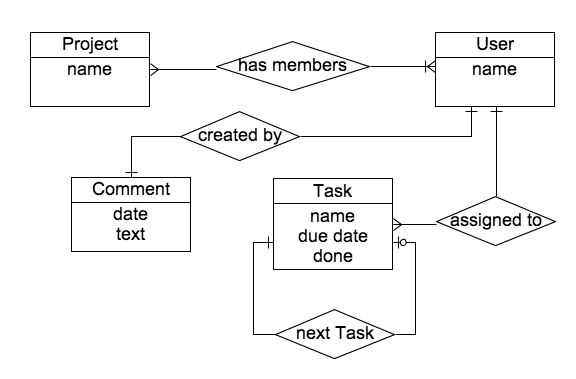
\includegraphics[width=0.8\textwidth]{img/tasks-schema}
\caption{A collaborative Task Manager's data model}
\label{fig:tasks-data-model}
\end{figure}

\section{Requirements}
\label{sec:requirements}
From the application scenarios we can derive a set of requirements for a synchronization solution.\\
The listed requirements resemble the goals set for the Bayou architecture back in 1994 \cite{Demers:1994vj}. 
Bayou had already proposed a distributed architecture with multiple devices acting as servers.
At that time the computational capabilities of mobile devices were very limited.
Today even smartphones have more storage and stronger CPUs than most servers in 1994.
Therefore pairwise synchronization should not only be possible between servers but also between mobile devices directly.

\subsection{Flexible Data Model Support}
A synchronization engine that is useful for a broad range of applications has to be able to deal with different data models. There is no magic algorithm that produces a perfect solution for an existing application.
Synchronization can happen with increasing levels of sophistication depending on the level of structural awareness of an application's data.\\
A ``dumb'' engine would have no awareness of an app's data model at all - it simply sees the entire application data as one binary chunk.\\
A more clever solution would maybe have an understanding of entities like Projects, Tasks or Comments and would see the entity instances as binary data.\\
It could get even finer grained and break up each entity instance into attributes which it recognizes as different pieces of data.\\
We see that \emph{synchronization granularity} is one key aspect when defining requirements.
The smallest pieces of information a synchronization engine can not break up further we call \emph{atoms}.
Atoms are usually aggregated into larger structures we call \emph{objects}.
A Task instance could be treated as an object which composes the title and due date attributes as atoms.\\
In order to be useful a synchronization engine does not need perfect understanding of the data to be synchronized.
Popular applications like Dropbox can provide useful synchronization of files without having any semantic understanding of their content.
For Dropbox each file is an atom - if a user adds a paragraph to a Word document, Dropbox only recognizes a change of the entire file.
This means if two users concurrently modify the same document at different places, Dropbox has no way to merge the changes correctly and will trigger a conflict.\\
Version control systems like git are usually more sophisticated - git treats each line in a file as an atom and can therefore often successfully merge concurrent changes.
Git still does not have any syntactic or even semantic awareness of the code that is written in the files it synchronizes.
So if there are concurrent edits, git can not guarantee that merges are syntactically or semantically correct.
Despite this seemingly low level of structural awareness, git is used very successfully in large software projects.\\

The data model of our application scenario is relatively simple but covers most of the modeling aspects the average mobile application needs:

\begin{itemize}
\item Entities and Instances
\item (Ordered) Collections
\item Attributes
\item Relationships (one to one, one to many, many to many)
\end{itemize}

This set of modeling elements is represented in many client-side application frameworks like Ember.js, Backbone or Angular.
If we can support synchronizing data with this type of schema it will make integration with existing frameworks fairly trivial.\\
We therefore require that the synchronization engine needs to have a structural awareness of at least the listed modeling components.

\subsection{Optimistic Synchronization}
As we have seen in the application scenario it is necessary that objects are editable on multiple devices even if they are not connected to a network.
Edits should be allowed concurrently to not block users from doing their work.
This implies that there can not be a central locking mechanism that controls when users can synchronize their data for offline usage.
We therefore trade strict consistency for availability of the data.\\
Synchronization happens in an optimistic manner which means that we assume that temporarily inconsistent data will rarely lead to problems.

\subsection{Eventual Consistency}
The sequence of states an object goes through as its edited is called its \emph{history}.
The history forms a directed graph with each state except the intial state having at least one ancestor.
The \emph{current state} is the one that has no descendants.
As edits can be made on different devices concurrently there can be multiple \emph{current states} at a time.
If an object has multiple current states we refer to them as \emph{branches}.\\
Our goal is to guarantee that after a finite number of synchronization events the object will eventually converge to the same state across all devices.\\
This trade-off is enforced by the \emph{CAP-Theorem} which states that it is impossible to have strong consistency combined with partition tolerance \cite{Gilbert:2002uw}.\\
Most mobile applications do not require strong consistency - the offline availability of data is usually a more important factor when judging the user experience. 

\subsection{Causality Preservation and Conflicts}
If an object diverges into multiple branches it will have to be reconciled during the synchronization process.
When we receive states from a remote device we need to reason about how we can apply them to our own edit history.\\
The \emph{happens-before} relationship defined by Lamport in \cite{Lamport:1978tr} helps to reason about this problem in an intuitive way.
A state \emph{a} that \emph{happened before} state \emph{b} refers to the fact that the edits that led to \emph{b} could have been affected by \emph{a}.
It is not necessarily related to the actual time of the edits that led to \emph{a} and \emph{b} as we can see in the following example:\\

Lets assume Rita and Allen work on the same object with their respective devices.
The object has the initial state \emph{a}.

\begin{itemize}
\item 9:00 AM: Rita makes an edit to the object which leads to state \emph{b}.
\item 9:30 AM: Allen synchronizes with Rita and edits which leads to state \emph{c}.
\item 10:00 AM: Rita is offline and can not synchronize. She edits the object at state \emph{b} leading to state \emph{d}. 
\end{itemize}

As Allen has seen state \emph{b} when making his edit, state \emph{b} \emph{happened before} state \emph{c}.\\
Rita has not seen state \emph{c} when making her edit.
Although the time of her edit is after Allen's edit there is no \emph{happened-before} relationship between state \emph{c} and \emph{d}.\\
On the next synchronization between Allen and Rita the system needs to identify this lack of causality as a \emph{conflict}.\\
While this example is simple, the identification of conflicts among a large group of collaborators can be non-trivial.\\
Depending on the level of understanding the synchronization engine has on the data there are strategies to resolve conflicts automatically.
The engine should be designed in a way that conflict resolution strategies can be ``plugged-in''.
If no automatic resolution is possible the application should be able to present the conflict to the user and let him manually resolve it.

\subsection{Flexible Network Topologies}
A traveling user who works with multiple mobile devices needs to be able to sychronize data without requiring internet access.
The synchronization engine should therefore be designed to handle peer-to-peer connections.\\
Even in an office environment where users exchange large amounts of data a direct connection can be significantly faster than doing a round-trip through a server on the internet.\\
For this setting a \emph{hybrid architecture} with local servers in the company network could be an interesting alternative.\\
The local servers could provide fast synchronization among users inside the office while a remote server on the internet provides synchronization with users working from home.\\
The local and remote servers are synchronizing in a peer-to-peer topology while the users interact with them in a client-server setup.\\
This gives us a hierarchical architecture which is both able to exploit the different levels of network speed and guarantee a higher state of consistency through the centralized servers.\\

The protocol used for synchronization should be generic enough to adapt to these different network setups.

\subsection{Integration with Existing Application Logic}
Most popular operating systems for mobile devices impose restrictions on the kind of software that can be installed.
Even if these limitations can be circumvented it provides a huge barrier to the install process of an app if external software is required.\\
For mobile applications it is therefore crucial that they can embed all their dependencies in the binary.
The synchronization engine should therefore be designed as an embeddable library.\\
Further it is important that the interfaces are designed to be as unintrusive into the application logic as possible.\\

A state based synchronization strategy is required to ease the integration process. The low-level aspects of \emph{update detection}, \emph{update propagation} and \emph{reconciliation} should be abstracted away from the application developer as much as possible.\\
At the same time the developer needs to be able to supply the logic for aspects of the synchronization that can not be solved generically. These include data model definition, conflict handling and technical aspects of messaging.

\section{Architecture of CouchDB}
CouchDB is a document-oriented database known for its data synchronization feature.
It currently is a popular tool for master-less synchronization directly between devices.\\
With multiple implementations being available for server, smartphone or in-browser deployment it seems like an excellent fit for our requirements.\\

The original implementation of CouchDB exposes an HTTP interface for all interactions with the database.
This makes it possible to write web applications directly targeting CouchDB as the server, eleminating any middleware in between.\\
If an application developer is able to design his application within the constraints of CouchDB being the only backend, it is called a \emph{CouchApp}.\\
CouchApps have the interesting property of being completely replicatable between CouchDB instances.
So an entire working application can be deployed to a device just by replicating it from a remote CouchDB instance.\\
Unfortunately only few applications get by with CouchDB being the only backend required.\\

With \emph{PouchDB} there has recently emerged a CouchDB implementation inside the browser in pure JavaScript.
It makes use of HTML5's IndexedDB as the storage layer and can therefore be included into a web application without requiring any plugins.\\
PouchDB exposes a similar interface like CouchDB and can fully synchronize with an actual CouchDB instance on a server.\\

CouchDB's data model is relatively simple - it mainly supports the storage of JSON-documents.
Each document has an ID under which it can be efficiently retrieved and updated.\\
There is no query language like SQL available as the stored JSON-documents are not required to have any fixed schema.\\
If effecient access to documents based on some of its properties is required, CouchDB allows the definition of \emph{views}.
Views are created by providing a map and possibly a reduce function.
The map function is used to define an index, while the reduce function can be used to efficiently compute aggregates.\\

An important aspect of CouchDB is that all its operations are lockless.
It achieves this by writing all data to an append-only data structure therefore never updating any data in-place.
Every update of a document creates a new version of it - similar to how some version control systems operate.\\
On each write of a new version, CouchDB requires that the current version ID of the document is passed.
This guarantees that the client has read the current version before he is able to write any updates.
If two clients concurrently update the same JSON-document, the first update that reaches the database succeeds and thereby creates a new version ID.
The second concurrent update will therefore be rejected as the client did supply an outdated version ID.
CouchDB treats this as an update conflict and notifies the second client.
The second client can then review the changes of the first client, possibly merge it with his changes and re-send it with the correct version ID.
This concept is often referred to as \emph{Optimistic Locking}.\\

In the case of concurrent edits on two instances of the same database the conflict handling is more complex.
Concurrent writes can no longer be linearized through optimistic locking as the two database instances are possibly disconnected.\\
CouchDB solves this by applying concepts of \emph{Multi-Version Concurrency Control}.
Both instances can update the same documents thereby creating two conflicting versions.\\
All versions of a document point to its ancestor resulting in a version tree.
If the database instances synchronize each other both instances will end up with both conflicting versions of the document.\\
CouchDB uses a deterministic algorithm to choose one of the instances as a winner.
As this choice is random to the user of an application it is often not the desired result.
It is therefore possible to either pick a different conflicting version as the winner or merge both versions to a new revision.

\subsection{Synchronization Protocol}

\subsection{Fulfillment of Requirements}
As a schemaless database CouchDB at least supports the storage of any kind of data model.
Its awareness of the type of data is at the same time very low.\\
When synchronizing databases CouchDB treats every JSON-document as an \emph{atom}.
There is no way to give CouchDB an increased level of awareness of an application's data model.\\
Application developers are therefore forced to write a large amount of additional merging logic inside their application.\\
Flexible data model support is therefore given while it requires additional app-specific logic to cater for CouchDB's lack of structural awareness.\\

The CouchDB model of multi-version concurrency control fulfills the requirement of optimistic synchronization.\\
Concurrently edited data on multiple CouchDB instances is eventually consistent if synchronized with each other.\\
The optimistic locking mechanism combined with a document's version tree ensures causality preservation.

CouchDB's distributed synchronization protocol supports a broad range of network topologies.\\

To build a more suitable solution for our requirements we can build on most of CouchDB's design decisions.\\
The major room for improvement lies in stronger data model awareness thereby relieving the application developer of repetitive merging logic.\\
We will also investigate an alternative synchronization protocol by collecting additional meta data on edits.

\section{Architecture of Histo}
Based on the requirements and the evaluation of CouchDB we derive a new architecture for a practical synchronization solution.

\begin{itemize}
\item
  \textbf{No Timestamps}: state-based 3-way merging
\item
  \textbf{No Change Tracing}: change tracing is not necessary - support
  diff computation on the fly
\item
  \textbf{Data Agnostic}: leave diff and merge of the actual data to
  plugins
\item
  \textbf{Distributed}: synchronization does not require a central server
\item
  \textbf{Functional Design}: only implement the functional parts of synchronization -
  leave everything else to the application (transport, persistence)
\item
  \textbf{Sensitive Defaults}: have defaults that \emph{just work} but
  still support custom logic (e.g. for conflict resolution)
\item
  \textbf{Cross-Platform}: be available on every major platform through the use of Web Standards
\end{itemize}

\section{Technologies used for Implementation}
We describe implementation details like the technologies used, code structure and the testing framework to evaluate the system.

- everything web-based --> only way to be cross-platform
- client-side persistence with HTML5
- note on alternatives (Lua, native)

\section{Differencing and Merging of Data Models}
- explain diff, merge and patch

- implement diff, merge and patch logic for primitive data structures
  -> use them to recursively model complex data structures

- ensure conflicts are made explicit

\subsection{Sets}
\subsection{Ordered Lists}
\subsection{Ordered Sets}
\subsection{Dictionaries}
used for object collections in data models
\subsection{Ordered Dictionaries}
most common for managing ordered object collections in data models
can be modeled with dictionary and ordered set/list
\subsection{Trees}
- tree as an example for composite data model
- efficient child tree pointers like in git

\subsection{Composite Data Structures}
- show how to represent complex data models as composite data structures

\section{Storing and Commiting Changes}
As syncing is state based we need to track the history of edits on each client.\\Each client has his own replica of the database and commits
data locally.\\On every commit we create a commit object that links both
to the new version of the data and the previous commit.\\

- use content-adressable store

- only store changes and reference unchanged data through hashs --> like git

- commit links to data and parent commit

\section{Differencing Across Commits}
- Most Recent Common Ancestor algorithm used for finding common commit of clients

- walk commit graph until MRCA

- recursive application of MRCA on every fork in graph

- implementation as separate module

\section{Synchronization Protocol}
Synchronization always happens from a \emph{Source} node to a \emph{Target} node.
If it is run simultaneously with Source and Target exchanged, it keeps both nodes in sync with each other.\\
The algorithm is designed to be able to run independently of the Source or Target.
It could be implemented as a separate application possibly even running on a different device - as long as it has access to both the Source and Target node.\\
The Synchronizer could be run in regular intervals or explicitly triggered by changes in the Source node.\\

The latest commit on a node we refer to as the \emph{head}.

Synchronization follows the following protocol:

\begin{enumerate}
\item Read all commit IDs since the last synced commit from Source and write them to Target.
\item Let the Target compute the common ancestor commit ID of Target's and Source's head.
\item Read all changed data since the common ancestor commit from Source and write to Target.
\item If the common ancestor equals the Source's head:\\
  The Source has not changed since the last synchronization. The Target's head is ahead of Source.\\
  The algorithm can stop here.
\item If the common ancestor equals the Target's head:\\
  The Target has not changed since the last synchronization.\\
  The Source's head is ahead of Target.\\
  We can fast-forward the Target's head to Source's head.
\item If the common ancestor is neither the Source's nor the Target's head:\\
  Both Source and Target must have changed data since the last synchronization.\\
  We run a three-way merge of the common ancestor, Source's head and Target's head.\\
  We commit the result as the new head to Target.
\end{enumerate}

This protocol is able to minimize the amount of data sent between synced
stores even in a distributed, peer-to-peer setting.\\

Updating the Target's head uses optimistic locking.
To update the head you need to include the last read head in your request.
So both the fast-forward operation or the commit of a merge result can be rejected if the Target has been updated in the meantime.
If this happens the Synchronizer simply has to re-run the algorithm.\\

We can express the protocol in pseudo-code as shown in listing \ref{sync-protocol}.

\begin{lstlisting}[caption=Synchronization Protocol, label=sync-protocol]

commitIDsSource = source.getCommitIDsSince(lastSyncedCommit)

target.writeCommitIDs(commitIDsSource)

commonAncestor = target.getCommonAncestor(target.head, source.head)

changedData = source.changedDataSince(commonAncestor)

target.writeData(changedData)

if (commonAncestor == source.head)
  // do nothing
else if (commonAncestor == target.head)
  target.setHead(source.head)
else
  commonAncestorData = target.getData(commonAncestor)
  sourceHeadData = source.getData()
  targetHeadData = target.getData()
  mergedData = three-way-merge(commonAncestorData, sourceHeadData, targetHeadData)
  // commit object linking commit data with its ancestors:
  commitObject = createCommit(mergedData, [source.head, target.head])
  target.commit(commitObject)

\end{lstlisting}

\section{Handling Conflicts}

\section{Optimizations}
Only keep limited history.

Clients who are disconnected for too long have to fetch redundant data.

Ideal case: remember until oldest head of nodes.

\section{Integration with Application Logic}
- demonstrate how to interface with standard MVC frameworks like Backbone, Ember.js

